\documentclass{article}
\usepackage{
	amsmath,			% Math Environments
	amssymb,			% Extended Symbols
	enumerate,		    % Enumerate Environments
	graphicx,			% Include Images
        minted,
        caption,
        subcaption
}

\title{MAT3100 - Oblig 1}
\author{August Femtehjell}
\date{February 2024}

\renewcommand{\thesection}{Oppgave \arabic{section}}
\renewcommand{\thesubsection}{\arabic{section}\alph{subsection})}
\renewcommand{\thesubsubsection}{Besvarelse}

\title{MAT1020 - Oblig 1\\Matematikk og bærekraftig forvaltning}
\author{August Femtehjell}
\date{March 2024}

\begin{document}

\maketitle

\section{}
I denne oppgaven skal du gjøre en statistisk analyse av kapasitetsfaktordataene.

\subsection{}
Plot alle dataseriene (gjerne som illustrative utsnitt av tidsseriene), og se om det er forskjeller mellom årstidene. Hva kan du si om solkraft nord og sør i Europa og vindkraft på de forskjellige stedene i Norge?

\subsubsection{}

\begin{figure}
\centering
\begin{subfigure}{.5\textwidth}
  \centering
  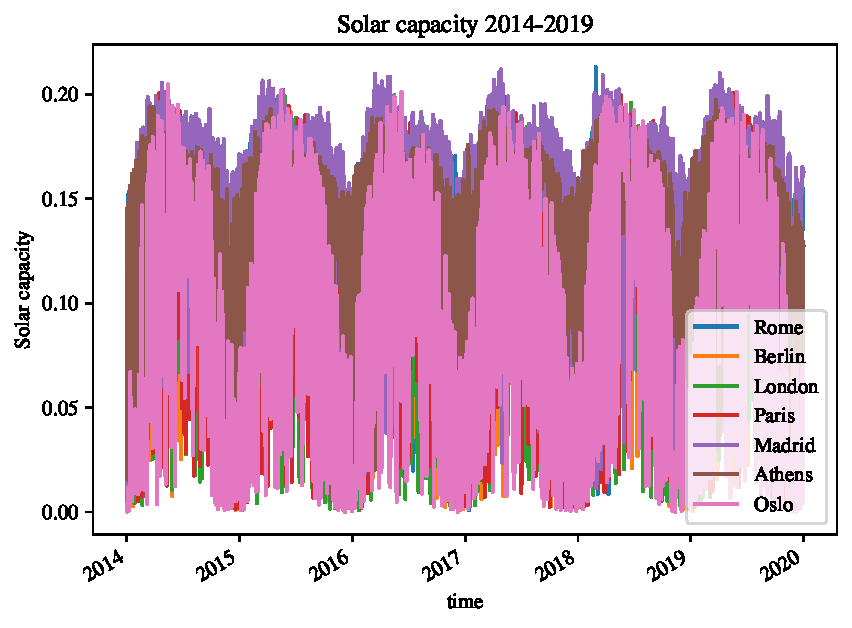
\includegraphics[width=.5\linewidth]{oblig/figures/Solar/Solar capacity 2014-2019.pdf}
  \caption{A subfigure}
  \label{fig:sub1}
\end{subfigure}%
\begin{subfigure}{.5\textwidth}
  \centering
  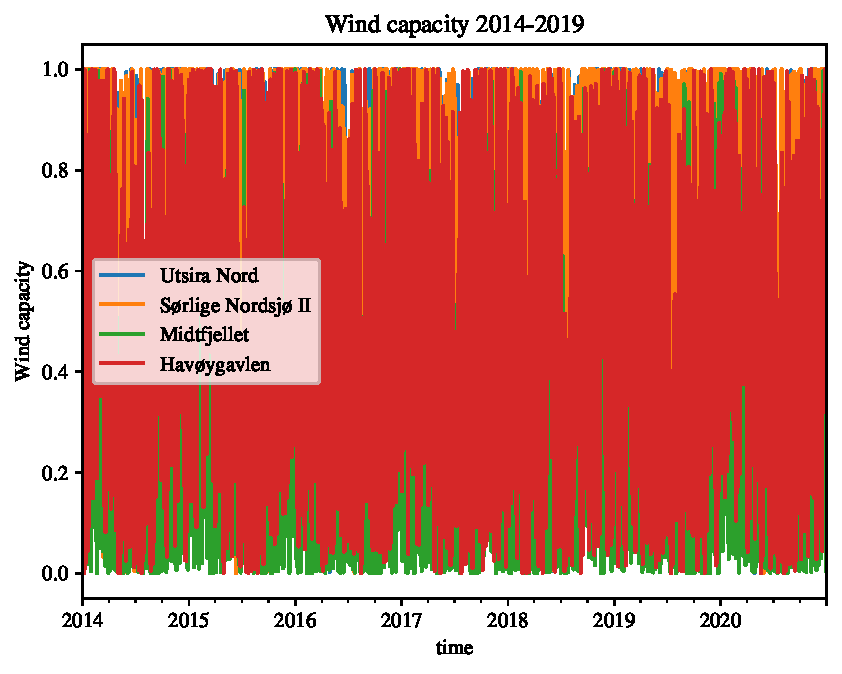
\includegraphics[width=.5\linewidth]{oblig/figures/Wind/Wind capacity 2014-2019.pdf}
  \caption{A subfigure}
  \label{fig:sub2}
\end{subfigure}
\caption{A figure with two subfigures}
\label{fig:test}
\end{figure}

\begin{figure}[h]
    \centering
    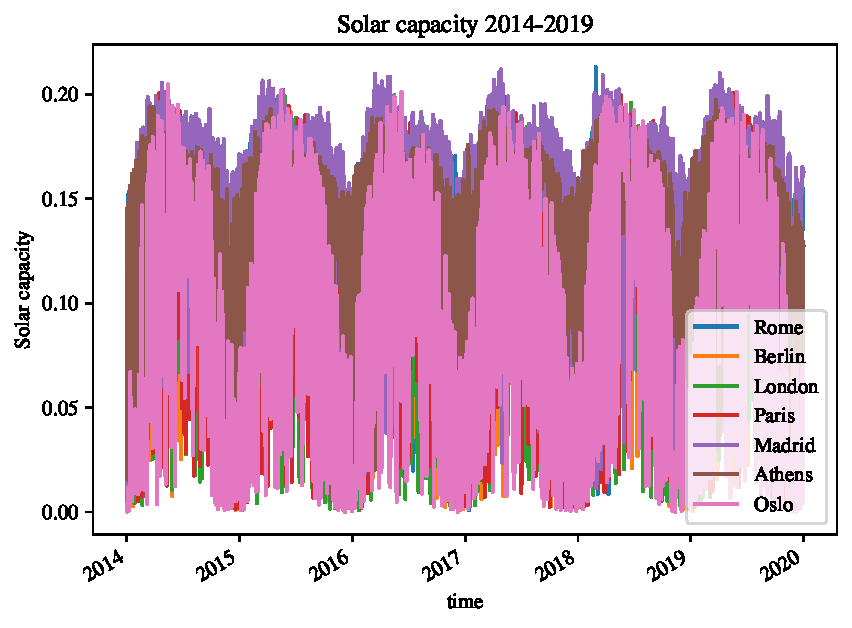
\includegraphics[width=0.5\textwidth]{oblig/figures/Solar/Solar capacity 2014-2019.pdf}
    \caption{Solkapasitet for perioden 2014-2019.}
    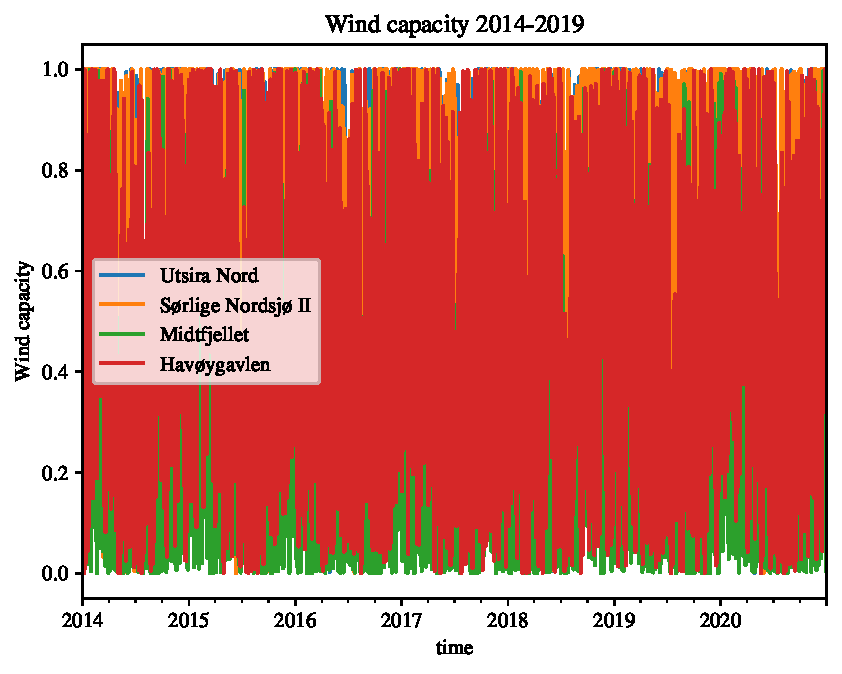
\includegraphics[width=0.3\textwidth]{oblig/figures/Wind/Wind capacity 2014-2019.pdf}
    \label{fig:total_solar}
\end{figure}

\subsection{}
Finn gjennomsnittlig kapasitetsfaktor for hver sol- og vind-dataserie. Husk å omforme sol-dataene til representative daglige verdier.

\subsection{}
Finn varians og standardavvik for kapasitetsfaktorene i hver lokasjon og hver teknologi (det vil si, sol og vind)

\subsection{}
Finn kovariansen til kapasitetsfaktorene mellom lokasjoner for vind. Hva blir korrelasjonene?

\subsection{}
Finn kovariansen til kapasitetsfaktorene mellom lokasjoner for sol. Hva blir korrelasjonene?

\subsection{}
Finn varians-kovariansmatrisen for kapasitetsfaktorene til sol og for kapasitetsfaktorene til vind.

\end{document}
